\documentclass[border=10pt]{standalone}
\usepackage[svgnames]{xcolor}
\usepackage{amsmath}
\usepackage{pgfplots}
\pgfplotsset{compat=newest}
\usepackage[sfdefault]{FiraSans}
\usepackage{FiraMono}
\renewcommand*\familydefault{\sfdefault}
\begin{document}
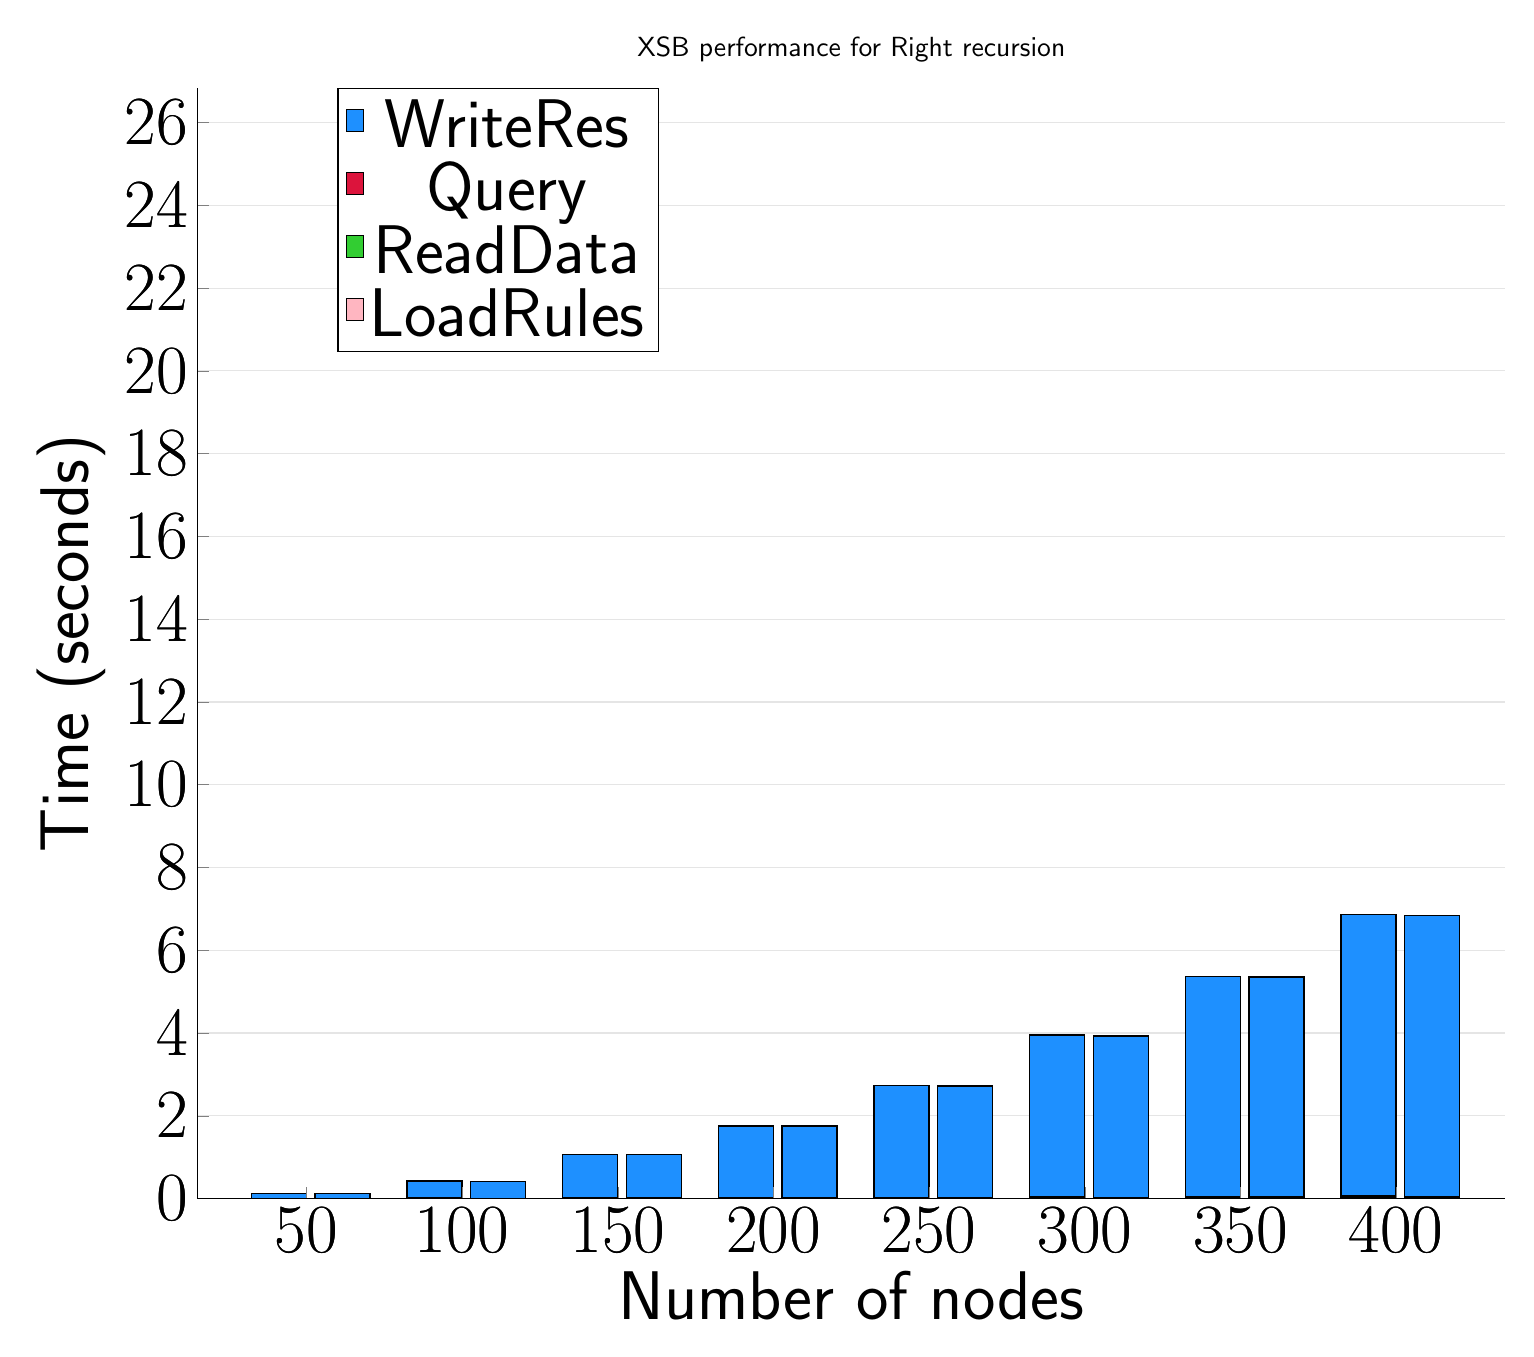
\begin{tikzpicture}
\begin{axis}[
   ybar stacked,
   title={XSB performance for Right recursion},
   bar shift=-10pt,
   width=1.5\textwidth,
   bar width=0.7cm,
   ymajorgrids, tick align=inside,
   major grid style={draw=gray!20},
   xtick=data,
   ymin=0, ymax=26.83928736050924,
   axis x line*=bottom,
   axis y line*=left,
   enlarge x limits=0.1,
   legend style={
       at={(0.23, 1)},
       anchor=north,
       legend columns=1,
       font=\Huge,
   },
   ylabel={Time (seconds)},
   xlabel={Number of nodes},
   label style={font=\Huge},
   tick label style={font=\Huge},
]
\addlegendimage{fill=DodgerBlue, draw=black, line width=0.2pt}
\addlegendentry{WriteRes}
\addlegendimage{fill=Crimson, draw=black, line width=0.2pt}
\addlegendentry{Query}
\addlegendimage{fill=LimeGreen, draw=black, line width=0.2pt}
\addlegendentry{ReadData}
\addlegendimage{fill=LightPink, draw=black, line width=0.2pt}
\addlegendentry{LoadRules}
\addplot +[fill=LightPink, draw=black, line width=0.5pt] coordinates {
    (50, 0.005055983861287434)
    (100, 0.005007743835449216)
    (150, 0.00504000981648763)
    (200, 0.0050099690755208365)
    (250, 0.00483504931131999)
    (300, 0.00478839874267578)
    (350, 0.005221366882324216)
    (400, 0.004748980204264323)
};
\addplot +[fill=LimeGreen, draw=black, line width=0.5pt] coordinates {
    (50, 0.0017970403035481766)
    (100, 0.00242296854654948)
    (150, 0.0033152898152669238)
    (200, 0.003983418146769206)
    (250, 0.0043122768402099635)
    (300, 0.005172014236450196)
    (350, 0.0057286421457926435)
    (400, 0.006661017735799153)
};
\addplot +[fill=Crimson, draw=black, line width=0.5pt] coordinates {
    (50, 0.0008396307627360026)
    (100, 0.00316770871480306)
    (150, 0.00803510348002116)
    (200, 0.014649709065755233)
    (250, 0.019016106923421233)
    (300, 0.0292486349741618)
    (350, 0.03784998257954917)
    (400, 0.050400575002034494)
};
\addplot +[fill=DodgerBlue, draw=black, line width=0.5pt] coordinates {
    (50, 0.11146871248881034)
    (100, 0.4165335496266683)
    (150, 1.0558448632558222)
    (200, 1.730156898498535)
    (250, 2.6974798838297525)
    (300, 3.9151123364766414)
    (350, 5.319701353708904)
    (400, 6.800863742828369)
};
\end{axis}
\begin{axis}[
   ybar stacked,
   bar shift=13pt,
   width=1.5\textwidth,
   bar width=0.7cm,
   ymajorgrids, tick align=inside,
   major grid style={draw=none},
   xtick=data,
   ymin=0, ymax=26.83928736050924,
   axis x line*=none,
   axis y line*=none,
   enlarge x limits=0.1,
   label style={font=\Huge},
   tick label style={font=\Huge},
]
\addplot +[fill=LightPink, draw=black, line width=0.5pt] coordinates {
    (50, 0.005037)
    (100, 0.0032913333333333358)
    (150, 0.00409933333333333)
    (200, 0.003981333333333333)
    (250, 0.004285333333333333)
    (300, 0.0028359999999999995)
    (350, 0.005168)
    (400, 0.004040666666666667)
};
\addplot +[fill=LimeGreen, draw=black, line width=0.5pt] coordinates {
    (50, 0.0017973333333333333)
    (100, 0.00161733333333333)
    (150, 0.0029876666666666667)
    (200, 0.003465666666666667)
    (250, 0.004220333333333333)
    (300, 0.0028613333333333334)
    (350, 0.00570166666666667)
    (400, 0.006560666666666666)
};
\addplot +[fill=Crimson, draw=black, line width=0.5pt] coordinates {
    (50, 0.0008396666666666643)
    (100, 0.002362)
    (150, 0.008035333333333337)
    (200, 0.011458000000000001)
    (250, 0.013287666666666665)
    (300, 0.022194333333333333)
    (350, 0.032025)
    (400, 0.034131666666666664)
};
\addplot +[fill=DodgerBlue, draw=black, line width=0.5pt] coordinates {
    (50, 0.11081400000000001)
    (100, 0.40663000000000005)
    (150, 1.052831)
    (200, 1.7317893333333334)
    (250, 2.700089333333333)
    (300, 3.902504)
    (350, 5.308592333333333)
    (400, 6.7920343333333335)
};
\end{axis}
\end{tikzpicture}

\end{document}
